\documentclass{report}
\usepackage[utf8]{inputenc}
\usepackage[T1]{fontenc}
\usepackage{longtable}
\usepackage{graphicx}
 \usepackage{array}
 \usepackage{caption}
 \usepackage{graphicx}
 \usepackage{rotating}
 \usepackage[usenames,dvipsnames]{xcolor}
\usepackage{tcolorbox}
\usepackage{tabularx}
\usepackage{array}
\usepackage{colortbl}
\usepackage{color}
\usepackage{multicol}
\tcbuselibrary{skins}
%\usepackage[italian]{babel}

%Disable all warnings issued by latex starting with "You have..."
\usepackage{silence}
\WarningFilter{latex}{You have requested package}
\pdfsuppresswarningpagegroup=1

%Bib
\usepackage[
backend=biber,
style=alphabetic,
sorting=ynt
]{biblatex}
\addbibresource{References.bib}

\usepackage{csquotes}
%\usepackage{natbib}


%Import
\usepackage{tabularx}
\usepackage{marvosym}
\usepackage{fancyvrb}
%\usepackage[usenames]{color}
\usepackage[hidelinks]{hyperref}
\usepackage{url}
\usepackage{graphicx}
\usepackage{xcolor}
\usepackage{amsmath,amsfonts,amssymb,amsthm,mathtools}
\usepackage{caption}
\usepackage{enumerate}
\usepackage{multicol}
\usepackage{subcaption}
\usepackage{float}
\usepackage{indentfirst}
\usepackage{tocloft}
\usepackage{ifthen}
%\usepackage[most]{tcolorbox}
\usepackage{pgfplots}
%\usepackage{Style/pgfplotsthemetol}
\pgfplotsset{compat=1.16}
\usepackage{listings}
\definecolor{lstgrey}{rgb}{0.94,0.95,1}
\lstset{
    language=python,
    backgroundcolor=\color{lstgrey},
    frame=single,
    rulecolor=\color{lstgrey}, % make frame "invisible"
    captionpos=t,
    tabsize=2,
    numberbychapter=false,
    showstringspaces=false,
    basicstyle=\footnotesize,
    breaklines=true,
}
%LINK CLICCABILI
\hypersetup{
    colorlinks = true,
    linkcolor = .,
    citecolor = {blue},
    linkbordercolor = {white},
    urlcolor = {blue},
}
%TABELLE TBCOLORBOX
\tcbset{
        enhanced,
        colback=red!5!white,
        boxrule=0.1pt,
        colframe=red!75!black,
        fonttitle=\bfseries
       }
       
%TAB2
\newcolumntype{Y}{>{\raggedleft\arraybackslash}X}

\tcbset{tab1/.style={fonttitle=\bfseries\large,fontupper=\normalsize\sffamily,
colback=yellow!10!white,colframe=red!75!black,colbacktitle=Salmon!40!white,
coltitle=black,center title,freelance,frame code={
\foreach \n in {north east,north west,south east,south west}
{\path [fill=red!75!black] (interior.\n) circle (3mm); };},}}

\tcbset{tab2/.style={enhanced,fonttitle=\bfseries,fontupper=\normalsize\sffamily,
colback=yellow!10!white,colframe=red!50!black,colbacktitle=Salmon!40!white,
coltitle=black,center title}}

%PATH IMMAGINI
%\graphicspath{{Images/}{DrawIo/}}
\newcommand{\emailaddr}[1]{\href{mailto:#1}{\texttt{#1}}}
%QandA
\usepackage{enumitem}
\newenvironment{QandA}{\begin{enumerate}[label=\bfseries\alph*.]\bfseries}
                      {\end{enumerate}}
\newenvironment{answered}{\par\normalfont}{}

\title{\LARGE
    PROCESSO DI SVILUPPO \\
    \hrulefill \\
    \textbf{ISIQuiz} \\ 
    \hrulefill \\
}
\author{
    Gambaletta Daniele \\ \emailaddr{daniele.gambaletta@studio.unibo.it}
    \and
    Lirussi Igor \\ \emailaddr{igor.lirussi@studio.unibo.it}
    \and 
    Omiccioli Riccardo \\ \emailaddr{riccardo.omiccioli@studio.unibo.it} 
    \and 
    Teodorani Cecilia \\ \emailaddr{cecilia.teodorani@studio.unibo.it} 
    \\ \\ \\ 
}




\date{\today}


\begin{document}

\renewcommand{\labelenumii}{\arabic{enumi}.\arabic{enumii}}
\renewcommand{\labelenumiii}{\arabic{enumi}.\arabic{enumii}.\arabic{enumiii}}
\renewcommand{\labelenumiv}{\arabic{enumi}.\arabic{enumii}.\arabic{enumiii}.\arabic{enumiv}}

\maketitle
\tableofcontents

% CONTENUTI
    \chapter{Product Backlog}
Per una visione generale del progetto, di seguito vengono inserite le immagini del \href{https://github.com/orgs/ISIQuiz/projects/3/views/2}{product backlog by progress}. In particolare, queste indicano la chiusura delle varie user story all'interno degli sprint anche se esse sono state iniziate precedentemente. Ad esempio, l'interfaccia grafica è stata iniziata nello sprint 8, ma conclusa solo nel 10. Poiché ad una user-story non possono essere assegnati più sprint, essa appare solo nel suddetto Sprint Backlog, mentre i suoi refinement sono presenti anche negli altri.

\begin{figure}[H]
    \centering
    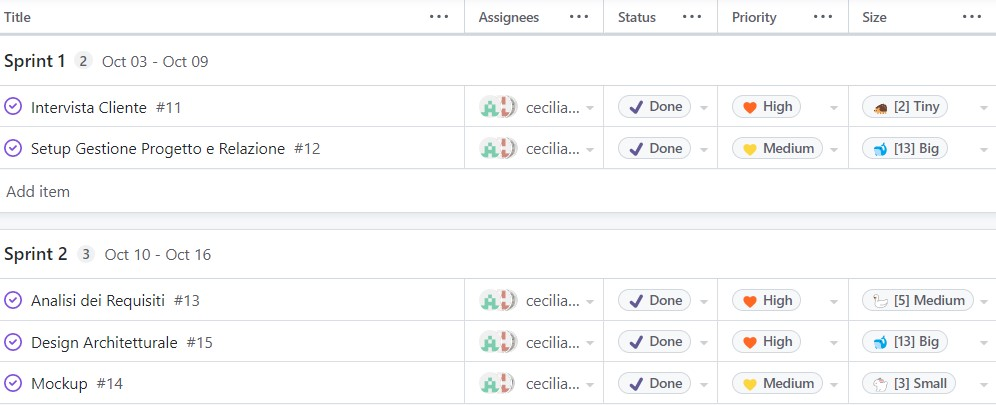
\includegraphics[width=\textwidth]{process/Img/sprint1_2.jpg}
    \label{fig:Sprint1_2}
\end{figure}
\begin{figure}[H]
    \centering
    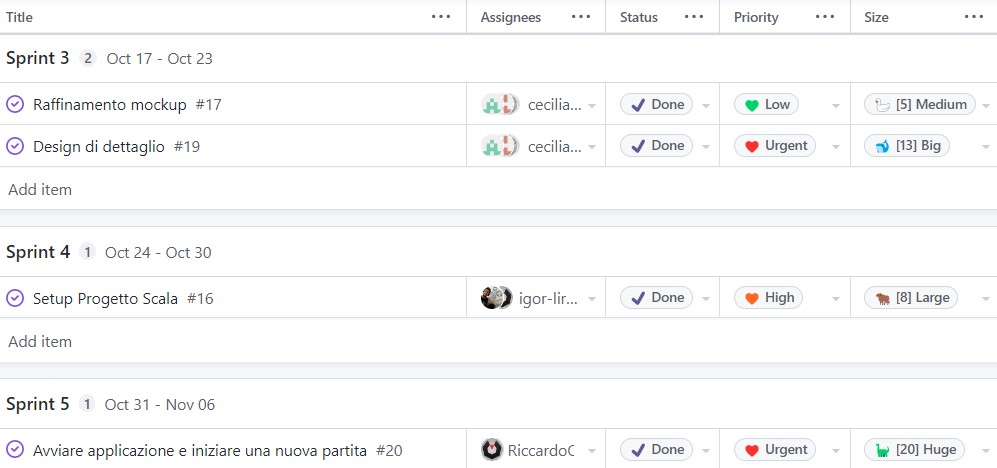
\includegraphics[width=\textwidth]{process/Img/sprint3_4_5.jpg}
    \label{fig:Sprint3_4_5}
\end{figure}
\begin{figure}[H]
    \centering
    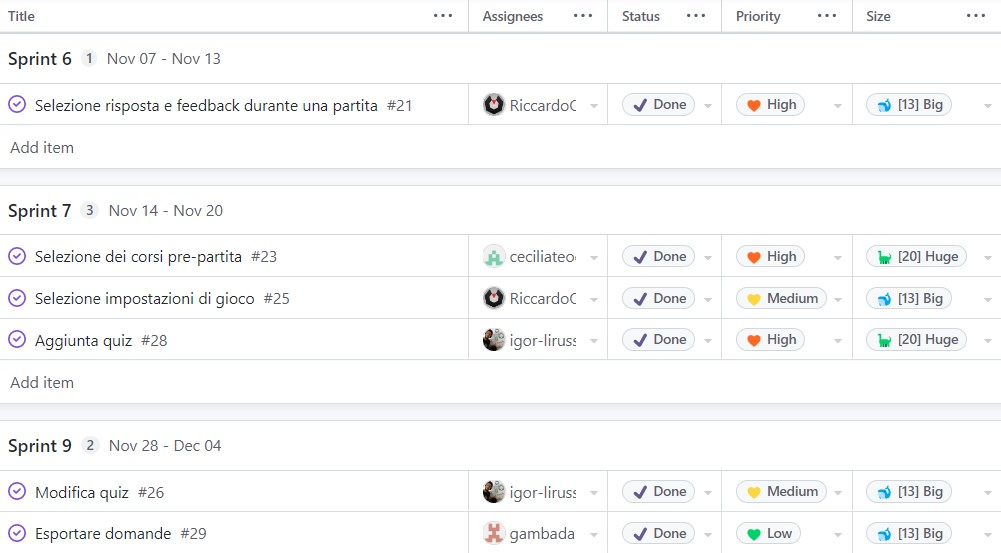
\includegraphics[width=\textwidth]{process/Img/sprint6_7_9.jpg}
    \label{fig:Sprint6_7_9}
\end{figure}
\begin{figure}[H]
    \centering
    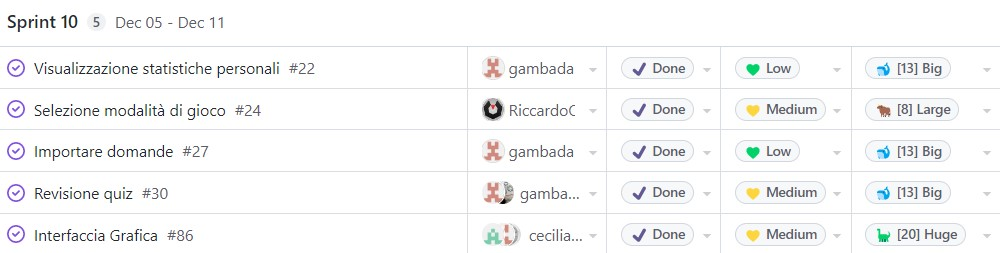
\includegraphics[width=\textwidth]{process/Img/sprint10.jpg}
    \label{fig:Sprint10}
\end{figure}

Nel capitolo finale \ref{chap:final-stats} sono invece inseriti dei grafici relativi al processo di sviluppo.
    \chapter{Sprint 0}

\section{Sprint Goal}
Sprint Goal


\section{Sprint Backlog}
%descrizione del refinement e immagine sprint backlog\textbf{}
descrizione del refinement


\section{Sprint Review}
%only this part is present also in the main report
%<*partPresentAlsoInReport>
Abbiamo studiato/implementato...
\paragraph{Deliverables} 
obiettivi raggiunti
\begin{itemize}
    \item uno
    \item due
    \item tre
\end{itemize}
%</partPresentAlsoInReport>


\section{Sprint Retrospective}
Sprint retrospective thoughts 
    \chapter{Meetings}

\section{Meetings}
\begin{itemize}
    \item 06/10/2022
        \begin{itemize}
            \item Decisa organizzazione generale
            \item Creato repository
        \end{itemize}
    \item 10/10/2022
        \begin{itemize}
            \item Intervista al domain expert
            \item Stesura requisiti utente, funzionali e non funzionali
            \item Stabilita definition of done
            \item Stabilito metodo di definizione dei pesi relativi ai task
        \end{itemize}
    \item 15/10/2022
        \begin{itemize}
            \item Review requisiti
            \item Creazione digramma classi e casi d'uso
            \item Definizione Ubiquitous Language
            \item Aggiunta e revisione mockup
        \end{itemize}
    \item 17/10/2022
        \begin{itemize}
            \item Riguardato il diagramma dei casi d'uso
            \item Sviluppato User Stories
            \item Creata la board di GitHub Projects
            \item Aggiornata la board di GitHub Projects
            \item Aggiornato il Gantt su Jira in base alle User Stories scelte
            \item Definizione task per lo Sprint 3
        \end{itemize}
    \item 20/10/2022
        \begin{itemize}
            \item Review dei mockup
            \item Schema relazione tra le view dei mockup
            \item Schema iniziale Model-View-Controller
        \end{itemize}
        
\end{itemize}


    \chapter{Final Statistics}
Statistiche finali sullo sviluppo e andamento del progetto corredate da grafici e tabelle
Da notare che le user stories appaiono sul product backlog solo sullo sprint che le ha concluse, ma possono essere state iniziate in precedenza. (I.E. L'interfaccia grafica è stata iniziata nello sprint 8 ma conclusa solo nel 10. Poichè ad una user-story, non possono essere assegnati più sprint appare solo nel suddetto Sprint Backlog, ma i suoi refinement sono presenti anche negli altri)

\nocite{*} % Includes all references from the `references.bib` file

\end{document}
